\documentclass[conference]{IEEEtran}
\usepackage[T1]{fontenc}
\usepackage[utf8]{inputenc}
\usepackage{cite}
\usepackage{amsmath}
\usepackage{graphicx}
\usepackage{tikz}
\usetikzlibrary{arrows.meta, positioning}
\usepackage{url}

\begin{document}

\title{When Does Self-Correction Help? An Empirical Study of\\
Feedback-Driven Repair in LLM Coding Agents\\
\textnormal{\large(Interim Report)}}

\author{
\IEEEauthorblockN{Luca Knierim}
\IEEEauthorblockA{
Department of Computer Science and Information Systems\\
University of Limerick\\
Limerick, Ireland\\
Student ID: 24403849}
}

\maketitle

\begin{abstract}
Large language model (LLM) agents increasingly review and revise their own output before returning it, a pattern commonly termed self-correction, self-refinement, or self-repair. Evidence for its effectiveness is mixed: some studies report substantial accuracy gains, whereas others find that, absent an external signal, models struggle to recognise their own errors and can degrade already-correct output while consuming additional time and tokens. Much of this evidence predates current-generation models and relies on benchmarks increasingly suspected of data contamination. This project investigates the cost-adjusted value of feedback-driven self-correction in LLM coding agents under controlled, isolated feedback conditions, using current models and a contamination-resistant benchmark. This interim report presents the background research, research questions, hypotheses, and methodology underpinning the project, together with the experimental platform built to date: a modular coding-agent architecture with a pluggable feedback interface, sandboxed code execution, and an evaluation harness instrumented to log correctness, token usage, and latency for every attempt. Empirical results are not yet available; a pilot run to estimate the cost of the full experiment is the immediate next step.
\end{abstract}

\begin{IEEEkeywords}
large language models, code generation, self-correction, software agents, empirical software engineering, benchmarking
\end{IEEEkeywords}

\section{Introduction}

A common design pattern lets an LLM agent review and revise its own output before returning it, a pattern referred to here as self-correction. Self-Refine and Reflexion presented iterative self-feedback as a general method for improving LLM output; Reflexion reported 91\% pass@1, the proportion of problems a model solves correctly on a single, unretried attempt, on the HumanEval coding benchmark, compared with 80\% for the previous state of the art~\cite{shinn2023,madaan2023}.

Subsequent work complicates this picture. Huang et al.\ found that LLMs struggle to self-correct their reasoning without external feedback, and that performance sometimes degrades after self-correction is attempted~\cite{huang2024}. Work specific to code generation shows that the type of feedback available to the agent matters: execution feedback from unit tests improved baseline accuracy by up to 12\%, and the format of that feedback was shown to affect the size of the gain~\cite{chen2024}. Olausson et al.\ found that once the cost of repair, in tokens and additional model calls, is taken into account, gains are often modest and sometimes absent; they argue that self-repair is bottlenecked by the model's ability to give useful feedback on its own code~\cite{olausson2024}. A critical survey by Kamoi et al.\ concluded that there is still no consensus on when LLMs can correct their own mistakes, that many studies use evaluations that overstate self-correction, and that self-correction works well when reliable external feedback is available~\cite{kamoi2024}.

Much of this evidence comes from 2023-era models evaluated on HumanEval~\cite{chen2021} and MBPP~\cite{austin2021}, benchmarks that Jain et al.\ argue now suffer from data contamination and saturation; they introduce LiveCodeBench, which collects new problems over time specifically to resist this~\cite{jain2025}. This project re-examines the cost-adjusted value of each feedback type on current models, using a contamination-resistant benchmark, and additionally measures how often self-correction breaks solutions that were initially correct, a question the cited studies do not isolate directly.

This project has three objectives. The first is to design and build a modular coding-agent platform with a pluggable feedback interface, a sandboxed execution environment, and an automated evaluation harness. The second is to compare four feedback conditions, no correction, intrinsic self-reflection, binary pass-or-fail feedback, and full execution feedback, on a contamination-resistant benchmark. The third is to determine whether, and under which conditions, self-correction improves correctness enough to justify its additional cost, including whether it ever degrades a solution that was already correct.

The project's contribution is twofold. As an empirical study, it provides an answer, grounded in current models, to a question the literature currently disputes. As an engineering artefact, it provides a reusable experimental platform that isolates the feedback variable cleanly enough to extend to further conditions or benchmarks. The remainder of this report reviews related work, states the research questions and hypotheses, describes the methodology and the platform built to date, and outlines the remaining project timeline.

\section{Related Work}

\subsection{Self-correction as a general method}

Self-Refine proposed that a model can improve its own output through iterative self-feedback, without additional training~\cite{madaan2023}. Reflexion extended this idea with a verbal reinforcement learning framework, in which an agent reflects on a failed attempt in natural language and uses that reflection on the next attempt; it reported 91\% pass@1 on HumanEval, against an 80\% prior state of the art~\cite{shinn2023}. Both papers treat self-feedback as broadly beneficial.

\subsection{Contrary evidence}

Huang et al.\ tested this assumption on reasoning tasks and found that current LLMs are often unable to identify errors in their own output without an external signal; self-correction without such a signal sometimes reduced accuracy relative to the original answer~\cite{huang2024}. This directly challenges the premise that reflection alone, absent ground truth, reliably improves output.

\subsection{The role of feedback type in code}

Work specific to code generation suggests the inconsistency between these findings is partly explained by what kind of feedback the agent receives. Chen et al.\ taught models to self-debug using execution feedback, unit test results together with the interpreter's error output, and reported accuracy improvements of up to 12\% over a no-feedback baseline, with the exact gain depending on the feedback format used~\cite{chen2024}. Olausson et al.\ evaluated self-repair once its cost, in additional tokens and model calls, was weighed against its benefit, and found the net gain was often small or absent; they attribute this to a bottleneck in the model's own ability to diagnose its mistakes rather than to the repair mechanism itself~\cite{olausson2024}. Kamoi et al.'s critical survey synthesises this literature and concludes that self-correction is effective specifically when reliable external feedback is available, and that evaluations lacking such feedback, or using contaminated benchmarks, tend to overstate how well models self-correct~\cite{kamoi2024}.

\subsection{Benchmark validity}

HumanEval~\cite{chen2021} and MBPP~\cite{austin2021} are the two benchmarks most of the cited work relies on. Jain et al.\ argue that both are now saturated and at risk of data contamination, since their problems have been public for several years and may appear, directly or in close paraphrase, in the training data of current models~\cite{jain2025}. They introduce LiveCodeBench, which draws problems from sources with verifiable release dates after a model's training cut-off, so that a reported result is less likely to reflect memorisation of a known solution~\cite{jain2025}.

\subsection{Positioning this project}

Three gaps motivate this project. First, the disagreement between Self-Refine or Reflexion and Huang et al.\ is largely unresolved on current, rather than 2023-era, models. Second, Olausson et al.'s cost-adjusted finding and Kamoi et al.'s feedback-availability account point to feedback type as the explanatory variable, but no single study compares no feedback, intrinsic reflection, and two levels of external feedback under otherwise identical conditions. Third, the degree to which self-correction degrades solutions that were already correct, as opposed to failing to fix incorrect ones, is mentioned as a risk but not measured directly in the cited work. This project addresses all three gaps using one platform and one contamination-resistant benchmark.

\section{Research Questions and Hypotheses}

\textbf{RQ1.} Does feedback-driven self-correction improve pass@1 correctness on a contamination-resistant coding benchmark when applied with current-generation models?

\textbf{RQ2.} Does the type of feedback available to the agent, none, intrinsic self-reflection, binary pass-or-fail, or full execution feedback, moderate the size of this effect?

\textbf{RQ3.} How often does self-correction degrade a solution that was correct before repair was attempted, and does this risk vary by feedback type?

\textbf{RQ4.} Once the additional tokens, latency, and repair rounds self-correction consumes are accounted for, does it remain worthwhile, or does its cost outweigh its benefit?

Four hypotheses follow from the literature reviewed in Section II.

\textbf{H1.} Full execution feedback will produce the largest improvement in pass@1 correctness among the four conditions, because it is the only condition that gives the agent the cause of a failure rather than only its presence~\cite{chen2024}.

\textbf{H2.} Intrinsic self-reflection, without an external correctness signal, will produce a negligible or negative net effect on correctness, consistent with Huang et al.'s finding that current models struggle to recognise their own errors unaided~\cite{huang2024}.

\textbf{H3.} Every correction condition will show a non-zero rate of degrading a solution that was correct before repair was attempted.

\textbf{H4.} Once token and latency cost are accounted for, the net benefit of self-correction will be smaller than pass@1 improvements alone suggest, consistent with Olausson et al.'s cost-adjusted finding~\cite{olausson2024}.

\section{Methodology}

\subsection{Platform architecture}

Figure~\ref{fig:architecture} shows the agent loop at the centre of the platform. The agent generates an initial solution to a problem, runs it in an isolated sandbox against the problem's hidden tests, and, for every condition except the no-correction baseline, repeats a repair round for a fixed number of iterations regardless of whether the current attempt already passes. The feedback strategy is the only part of this loop that differs between experimental conditions: it is implemented as a single interface with four interchangeable implementations, so that a condition changes only the information given to the model and nothing else about generation, execution, or logging.

\begin{figure}[htbp]
\centering
\resizebox{\columnwidth}{!}{%
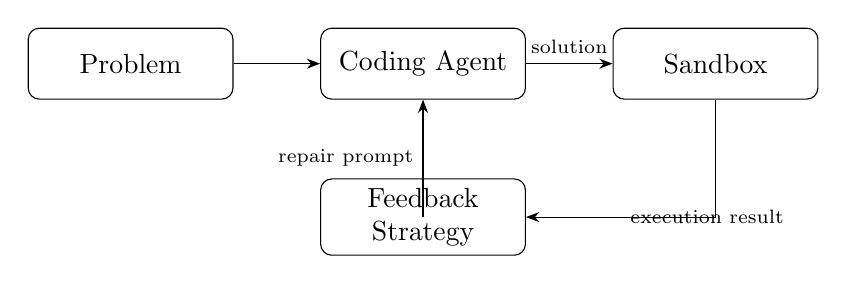
\begin{tikzpicture}[
  box/.style={draw, rounded corners, align=center, minimum height=0.9cm, minimum width=2.6cm},
  >=Stealth
]
  \node[box] (problem) {Problem};
  \node[box, right=1.1cm of problem] (agent) {Coding Agent};
  \node[box, right=1.1cm of agent] (sandbox) {Sandbox};
  \node[box, below=1.0cm of agent] (feedback) {Feedback\\Strategy};

  \draw[->] (problem) -- (agent);
  \draw[->] (agent) -- node[above, font=\scriptsize] {solution} (sandbox);
  \draw[->] (sandbox) |- node[right, font=\scriptsize, pos=0.75] {execution result} (feedback);
  \draw[->] (feedback) -| node[left, font=\scriptsize, pos=0.75] {repair prompt} (agent);
\end{tikzpicture}%
}
\caption{The agent loop. The feedback strategy is the sole experimental variable; the rest of the loop is shared by every condition.}
\label{fig:architecture}
\end{figure}

\subsection{Experimental conditions}

Four conditions are implemented. In the \emph{no-correction} condition, the agent makes a single attempt and never repairs it, establishing a baseline. In the \emph{self-reflection} condition, the agent is asked to review and, if necessary, revise its own solution, but is never told whether the previous attempt passed or failed, isolating the no-external-signal setting Huang et al.\ evaluate~\cite{huang2024}. In the \emph{binary} condition, the agent is told only whether its previous attempt passed or failed the hidden tests, with no further detail. In the \emph{execution} condition, the agent is told the pass-or-fail outcome together with the interpreter's error output or failing test result, isolating the setting Chen et al.\ evaluate~\cite{chen2024}. Repair rounds continue for all conditions but no-correction even after a correct attempt, so that H3 can be tested directly rather than inferred.

\subsection{Sandboxed execution}

A candidate solution must be run to be judged correct, but it is machine-generated and untrusted; executing it directly on a researcher's own machine would be reckless. The platform defines one sandbox interface with two interchangeable backends. The first isolates execution in a separate process, with a wall-clock timeout and a restricted environment; this works without additional setup but gives a weaker isolation guarantee. The second isolates execution inside a disposable Docker container with no network access and a fixed memory limit; this is the stronger guarantee and is used by default. The network restriction was verified directly: an attempt, from inside the sandbox, to open a socket to an external host fails in every case tested.

\subsection{Benchmarks}

HumanEval~\cite{chen2021} is used during development and for the pilot run described in Section VI, because it is small, well understood, and inexpensive to iterate on. LiveCodeBench~\cite{jain2025} is the primary benchmark for the full experiment, because its problems are drawn from sources with dates after current models' training cut-offs, which limits the risk that a reported result reflects a memorised solution rather than one the model actually derived, the concern Jain et al.\ raise against HumanEval and MBPP~\cite{jain2025}.

\subsection{Evaluation harness and metrics}

Every attempt in a trajectory, not only the final one, is logged to a structured store: whether it passed, wall-clock duration, input and output token counts, and, on failure, the interpreter's error output. This is necessary for three reasons. It is the only way to measure whether an initially correct solution was later broken, which answers RQ3. It is the only way to compute a cost-adjusted comparison between conditions, which answers RQ4, rather than a pass@1 comparison alone. It also allows the recorded data to be re-analysed later without repeating the model calls that produced it.

\subsection{Experimental design and planned analysis}

Each problem will be attempted under every condition, a repeated-measures design, so that a difference between conditions on a given problem cannot be attributed to the problem itself varying in difficulty between conditions. Pass@1 will be reported as a raw count over the number of problems attempted, alongside a percentage, rather than as a percentage alone, since a benchmark subset may be small relative to the full pool. Paired conditions, for example no-correction against execution feedback on the same problem set, will be compared using a statistical test appropriate to matched binary outcomes, such as McNemar's test; the exact test will be confirmed once pilot data indicate whether its assumptions hold.

\subsection{Ethical and practical considerations}

This project involves no human participants; the subjects under study are LLMs queried through an API, evaluated against publicly available, non-personal coding benchmark problems. Ethical approval under the Faculty's human-participants research process is therefore not required, consistent with Declaration 2 of the approved project proposal. The ethical consideration that does apply is the safe execution of untrusted, machine-generated code, addressed in Section~IV-C.

The primary practical constraint is API cost, since every repair round issues an additional model call; a pilot run on a small HumanEval subset, discussed in Section~VI, is planned to estimate the cost of the full experiment before it is run at scale. The second constraint is time, addressed by the remaining timeline in Section~VI.

\section{Work Completed to Date}

The platform described in Section IV has been implemented and is in active use for development testing. The agent loop and all four feedback strategies are implemented behind the interfaces described above. Each strategy is tested directly for the property its condition is defined by: the self-reflection strategy is verified never to read the sandbox's execution result, and the binary strategy is verified never to include the interpreter's error output in the message sent back to the model, so that the four conditions cannot silently leak information across their intended boundaries.

Both sandbox backends are implemented and tested, including the subprocess backend's timeout and the Docker backend's network isolation. An evaluation harness logs every attempt to a queryable store, recording pass-or-fail status, token counts, and latency, and a small command-line interface runs a batch of problems across a chosen set of conditions.

A continuous-integration pipeline enforces this work on every change before it is merged: an automated test suite, static type checking, a lint check, and a check that newly added code is itself covered by tests. At the time of writing, the test suite comprises 22 automated tests, covering the sandbox backends, each feedback condition's information boundary, code extraction from model output, experiment logging, and the command-line interface, all of which currently pass.

\section{Project Plan and Remaining Timeline}

The approved project proposal set out an eight-month plan. The first month, literature review and research design, and the second month, the core agent loop and sandboxed execution environment, are complete. The pluggable feedback system and evaluation harness, originally scheduled for the third month, are also complete, along with the continuous-integration pipeline described in Section V, which was not separately scheduled but supports every month that follows it.

The immediate next step is a small pilot run on HumanEval to estimate the per-condition cost of the full experiment. LiveCodeBench will then be integrated, completing the platform as proposed for month four. The full experiment will be run across all four conditions in months five and six, the results will be analysed statistically in month seven, and the dissertation, demonstration, and presentation will be completed in month eight.

\section{Conclusion}

At this stage, the project's contribution is a research design that isolates feedback type as a single variable, a working platform that implements and tests that design, and a set of hypotheses grounded directly in the literature reviewed in Section~II. No empirical findings are yet available; reporting any would be premature before the pilot run and the full experiment described in Section~VI have been carried out. The gap motivating this project, disagreement over when and whether self-correction helps, evaluated on current models and a contamination-resistant benchmark, remains open, and the next stage of this project is designed to close it.

\section*{Declaration on the Use of Generative AI}

Generative AI, specifically Claude Code, built on Anthropic's Claude model family, was used during this project under the express written permission of the supervisor, obtained by email. A copy of that email exchange is included as Appendix~A. The tool was used to discuss and implement the platform architecture described in Section~IV, including the agent loop, the four feedback strategies, both sandbox backends, the evaluation harness, and the continuous-integration pipeline; to assist in debugging, for example identifying a type error in the command-line interface's error-handling path; and to draft prose for this report, which was reviewed, edited, and is approved in full by the author. The author takes full responsibility for the content of this report and the code it describes.

\section*{Academic Integrity Declaration}

[Insert the University of Limerick's standard academic integrity and plagiarism declaration, signed and dated, as required for the interim submission.]

\section*{Acknowledgment}

The author thanks Chris Exton for his supervision of this project.

\bibliographystyle{IEEEtran}
\bibliography{refs}

\appendices
\section{Supervisor Email Authorising the Use of Generative AI}
[Insert a copy of the email exchange with the supervisor here before submission.]

\end{document}
